%% -*- latex-mode -*-
\begin{example}
  The formula $t \leq 2a \leq r \leq 2b+1 \leq t$ has no integer
  solution but a rational solution.  Introducing the branch $a\leq b
  \lor b < a$ leads to the theory conflicts $t\leq 2a \leq 2b \leq
  t-1$ and $r \leq 2b+1 \leq 2a-1 \leq r-1$ (note that $b<a$ is
  equivalent to $b+1 \leq a$).  The corresponding proof tree is given
  below.  The Farkas coefficients in the theory lemmas are given in
  parenthesis.  Note that the proof tree shows the clauses, i.\,e.,
  the negated conflicts.  A node with more than two parents denotes that
  multiple applications of the resolution rule are taken one after another.

  \centerline{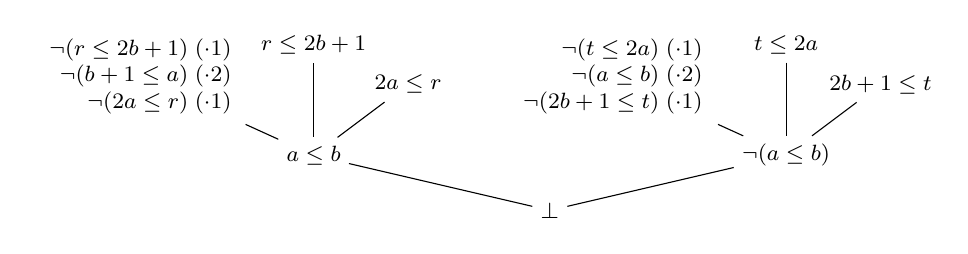
\begin{tikzpicture}\footnotesize
    \node (t2) at(0,0) {$\begin{array}{r}\lnot(r\le 2b+1)\;(\cdot 1)\\\lnot
        (b+1\le a)\;(\cdot 2)\\\lnot(2a\le r)\;(\cdot 1)\end{array}$};
    \node (t1) at(6,0) {$\begin{array}{r}
                          \lnot(t\le 2a)\;(\cdot 1)\\
                          \lnot(a\le b)\;(\cdot 2)\\
			  \lnot(2b+1\le t)\;(\cdot 1)
			  \end{array}$};
    \node (i21) at(2.2,.4) {$r\leq 2b+1$};
    \node (i22) at(3.4,-.1) {$2a\leq r$};
    \node (i11) at(8.2,.4) {$t\leq 2a$};
    \node (i12) at(9.4,-.1) {$2b+1\leq t$};
    \node (r2) at(2.2,-1) {$a\le b$};
    \node (r1) at(8.2,-1) {$\lnot(a\le b)$};
    \node (b) at(5.2,-1.7) {$\bot$};
    \draw (t1)-- (r1);
    \draw (i11)-- (r1);
    \draw (i12)-- (r1);
    \draw (t2)-- (r2);
    \draw (i21)-- (r2);
    \draw (i22)-- (r2);
    \draw (r1)-- (b);
    \draw (r2)-- (b);
  \end{tikzpicture}}

Now consider the problem of deriving an interpolant between $A\equiv t\le
2a\le r$ and $B\equiv r\le 2b+1\le t$.  We can obtain an interpolant by
annotating the above resolution tree with partial interpolants.  
To compute a partial interpolant for the theory lemma
$\lnot(r\le 2b+1) \lor \lnot(b+1\le a) \lor \lnot(2a\le r)$,
we purify the \emph{negated} clause according to the definition in
Section~\ref{sec:purification}, which gives
\[ r\le 2b+1  \land  x_1 \le a \land -x_1 + b + 1 \le 0 \land 2a\le r. \]
Then, we sum up the $A$-part of the conflict (the second
and fourth literal) multiplied by their corresponding Farkas coefficients.
This yields the interpolant $2x_1 \le r$.
Similarly, the negation of the theory lemma 
$\lnot(t\le 2a) \lor \lnot(a\le b) \lor  \lnot(2b+1\le t)$ is purified to
\[t\le 2a \land x_2+a\le 0 \land -x_2\le b \land  2b+1\le t,\]
which yields the partial interpolant $2x_2+t \le 0$.  
Note, that we have to introduce different variables for each literal.
Intuitively, the variable $x_1$ stands for $a$ and $x_2$ for $-a$.  
Using Pudl\'ak's algorithm we can derive the same interpolants for 
the clause $a\leq b$ resp.\ $\lnot (a\leq b)$.

For the final resolution step, the two partial interpolants 
$2x_1 \le r$ and $2x_2+t \le 0$ are combined into
the final interpolant of the problem.
Summing up these inequalities with $x_1=-x_2$ we get $t\le r$.  
While this follows from $A$, it is not
inconsistent with $B$.  We need an additional argument that, given $r=t$,
$r$ has to be an even integer.  This also follows from the partial
interpolants when setting $x_1=-x_2$: $t\leq -2x_2 = 2x_1 \leq r$.
\ifnewinterpolation
The final interpolant computed by our algorithm is 
$t \leq 2\floorfrac{r}{2}$.
\else
The final interpolant computed by our algorithm is 
$t \leq r \land (t \geq r \rightarrow t \leq 2\lfloor r/2\rfloor)$.
\fi

%Using the Strong-Weak-Interpolation lemma we have to find I3 such that
%(ALL x_1 x_2.   x_1 \le a --> 2x_1 \le r  
%           &&  x_2 +a \le 0 --> 2x_2 + t \le 0) --> I3
%and
%I3 --> (EX x_1 x_2. -x_1 + b + 1 \le 0 && 2x_1 \le r  
%                  ||  -x_2  \le b && 2x_2 + t \le 0)


In general, we can derive additional constraints on the variables
if the constraint resulting from summing up the two partial interpolants
holds very tightly. We know implicitly that $x_1=-x_2$ is an integer
value between $t/2$ and $r/2$.  If $t$ equals
$r$ or almost equals $r$ there are only a few possible values which we can
explicitly express using the division function as in the example above.
\ifnewinterpolation
We assume that the (partial) interpolant $F$ always has a certain
property.  There is some term $s$ and some constant $k$, such that
for $s > 0$ the interpolant is always false and for $s < -k$ the
interpolant is always true (in our case $s = t-r$ and $k = 0$). 
For a partial interpolant that still contains auxiliary variables $\vec x$,
we additionally require that $s$ contains them with a positive coefficient
and that $F$ is monotone on $\vec x$, i.\,e., $\vec x \geq \vec x'$ implies
$F(\vec x) \rightarrow F(\vec x')$.
\else
This leads to the general form $t-r\leq 0\land (t-r\geq
-k\rightarrow F)$.  In our example we have $k=0$ and $F$ specifies
that $r=t$ is even.
\fi
\end{example}

%%  LocalWords:  interpolant interpolants
